\section{Special Functions}
    There are many special functions that arise in diffraction
    theory. These are functions that can not be written in
    closed form via a combination of rational functions,
    trigonometric functions, logarithms, or exponentials.
    Usually such functions are defined as the solution to
    a particular differential equation, such as Bessel
    functions, or as the result of integrating a non-trivial
    function, such as Fresnel Integrals. Other times functions
    are defined as the inverse of a tricky algebraic equation,
    such that the Lambert $W$ function. We'll discuss these
    three functions, numerical calculations, and their
    applications.
    \subsection{The Fresnel Integrals}
        The Fresnel Sine and Cosine Integrals, which are
        usually denoted $S(x)$ and $C(x)$, respectively,
        occur naturally in the study of diffraction theory.
        By examining the \textit{Fresnel Kernel},
        and using a Taylor series approximation, one
        comes across the following integral:
        \begin{equation}
            F(x)=\int_{0}^{x}\exp(it^{2})\diff{t}
        \end{equation}
        Using Euler's Theorem, we can rewrite this as:
        \begin{equation}
            F(x)=\int_{0}^{x}\cos(t^{2})\diff{t}
                +i\int_{0}^{x}\sin(t^{2})\diff{t}
        \end{equation}
        The Fresnel Cosine and Sine Integrals are defined
        as the real and
        imaginary parts of this equation, respectively.
        \begin{ldefinition}{Fresnel Integrals}
            The Fresnel Sine and Fresnel Cosine, denoted
            $S(x)$ and $C(x)$, respectively, are real valued
            functions defined by:
            \par\hfill\par
            \vspace{-1ex}
            \begin{subequations}
                \begin{minipage}{0.49\textwidth}
                    \begin{equation}
                        S(x)=\int_{0}^{x}
                        \sin(t^{2})\diff{t}
                    \end{equation}
                \end{minipage}
                \hfill
                \begin{minipage}{0.49\textwidth}
                    \begin{equation}
                        C(x)=\int_{0}^{x}
                        \cos(t^{2})\diff{t}
                    \end{equation}
                \end{minipage}
            \end{subequations}
            \par
        \end{ldefinition}
        Graph of the Fresnel Sine and Fresnel Cosine
        functions are shown in
        Fig.~\ref{fig:Diff_Theory_Graphs_of_Sinx2_and_Cosx2}.
        \begin{figure}[H]
            \captionsetup{type=figure}
            \centering
            \begin{subfigure}[b]{0.49\textwidth}
                \centering
                \resizebox{\textwidth}{!}{%
                    \documentclass[crop,class=article]{standalone}
%----------------------------Preamble-------------------------------%
\usepackage{tikz}                       % Drawing/graphing tools.
\usetikzlibrary{arrows.meta}            % Latex arrows.
\newcommand*\diff{\mathop{}\!\mathrm{d}}
%--------------------------Main Document----------------------------%
\begin{document}
    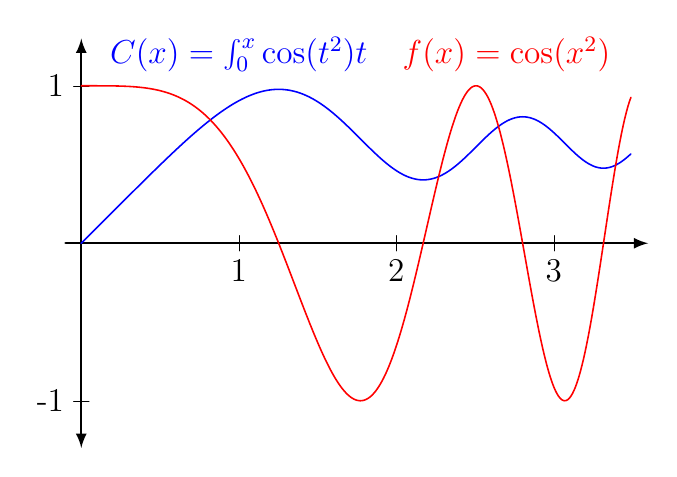
\begin{tikzpicture}[%
        >=latex,
        line width=0.2mm,
        line cap=round,
        scale=2
    ]
        \draw[->, black, thick] (-0.1, 0) to (3.6, 0);
        \draw[<->, black, thick] (0, -1.3) to (0, 1.3);
        \begin{scope}[%
            line width = 0.05mm,
            font=\large
        ]
            \draw (1, 0.05) to (1, -0.05) node[below] {1};
            \draw (2, 0.05) to (2, -0.05) node[below] {2};
            \draw (3, 0.05) to (3, -0.05) node[below] {3};
            \draw (0.05, 1) to (-0.05, 1) node[left] {1};
            \draw (0.05, -1) to (-0.05, -1) node[left] {-1};
            \node at (1, 1.2) 
                {$\textcolor{blue}{C(x)=\int_{0}^{x}\cos(t^{2})\diff{t}}$};
            \node at (2.7, 1.2) {$\textcolor{red}{f(x)=\cos(x^{2})}$};
        \end{scope}
        \draw[blue] (0.0, 0.0) to (0.01, 0.009999999989999783)
                               to (0.02, 0.01999999967999957)
                               to (0.03, 0.029999997570000502)
                               to (0.04, 0.039999989760001305)
                               to (0.05, 0.049999968750008845)
                               to (0.06, 0.0599999222400464)
                               to (0.07, 0.06999983193018723)
                               to (0.08, 0.07999967232062173)
                               to (0.09, 0.08999940951179344)
                               to (0.1, 0.09999900000462966)
                               to (0.11, 0.1099983895009161)
                               to (0.12, 0.11999751170388809)
                               to (0.13, 0.1299962871190949)
                               to (0.14, 0.13999462185565228)
                               to (0.15, 0.1499924064279761)
                               to (0.16, 0.15998951455814062)
                               to (0.17, 0.16998580197900762)
                               to (0.18, 0.17998110523830813)
                               to (0.19, 0.1899752405038796)
                               to (0.2, 0.19996800237028275)
                               to (0.21, 0.2099591626670576)
                               to (0.22, 0.21994846926890724)
                               to (0.23, 0.2299356449081313)
                               to (0.24, 0.23992038598965387)
                               to (0.25, 0.2499023614090435)
                               to (0.26, 0.2598812113739407)
                               to (0.27, 0.2698565462293629)
                               to (0.28, 0.2798279452873871)
                               to (0.29, 0.2897949556617517)
                               to (0.3, 0.29975709110796817)
                               to (0.31, 0.3097138308695744)
                               to (0.32, 0.31966461853120126)
                               to (0.33, 0.3296088608791891)
                               to (0.34, 0.3395459267705181)
                               to (0.35, 0.34947514601088253)
                               to (0.36, 0.3593958082427811)
                               to (0.37, 0.36930716184456436)
                               to (0.38, 0.3792084128414092)
                               to (0.39, 0.38909872382926997)
                               to (0.4, 0.39897721291290555)
                               to (0.41, 0.4088429526591272)
                               to (0.42, 0.418694969066499)
                               to (0.43, 0.42853224055275235)
                               to (0.44, 0.43835369696125703)
                               to (0.45, 0.44815821858795346)
                               to (0.46, 0.4579446352302023)
                               to (0.47, 0.46771172525908233)
                               to (0.48, 0.4774582147167299)
                               to (0.49, 0.487182776440374)
                               to (0.5, 0.49688402921479474)
                               to (0.51, 0.5065605369549924)
                               to (0.52, 0.5162108079209244)
                               to (0.53, 0.5258332939662359)
                               to (0.54, 0.5354263898229702)
                               to (0.55, 0.5449884324243203)
                               to (0.56, 0.5545177002675439)
                               to (0.57, 0.5640124128192319)
                               to (0.58, 0.5734707299651866)
                               to (0.59, 0.5828907515072299)
                               to (0.6, 0.592270516709329)
                               to (0.61, 0.6016080038954872)
                               to (0.62, 0.6109011301019069)
                               to (0.63, 0.6201477507860028)
                               to (0.64, 0.6293456595948895)
                               to (0.65, 0.6384925881960349)
                               to (0.66, 0.6475862061728191)
                               to (0.67, 0.6566241209877995)
                               to (0.68, 0.6656038780165191)
                               to (0.69, 0.6745229606547636)
                               to (0.7, 0.6833787905021972)
                               to (0.71, 0.6921687276253586)
                               to (0.72, 0.7008900709030388)
                               to (0.73, 0.7095400584570886)
                               to (0.74, 0.7181158681717404)
                               to (0.75, 0.72661461830455)
                               to (0.76, 0.7350333681920904)
                               to (0.77, 0.7433691190535345)
                               to (0.78, 0.7516188148952926)
                               to (0.79, 0.7597793435198523)
                               to (0.8, 0.7678475376419894)
                               to (0.81, 0.7758201761154937)
                               to (0.82, 0.7836939852735506)
                               to (0.83, 0.7914656403858894)
                               to (0.84, 0.7991317672357902)
                               to (0.85, 0.8066889438199938)
                               to (0.86, 0.814133702174525)
                               to (0.87, 0.8214625303293743)
                               to (0.88, 0.8286718743949371)
                               to (0.89, 0.8357581407830177)
                               to (0.9, 0.8427176985651446)
                               to (0.91, 0.8495468819708369)
                               to (0.92, 0.8562419930283709)
                               to (0.93, 0.8627993043504705)
                               to (0.94, 0.869215062067243)
                               to (0.95, 0.8754854889085183)
                               to (0.96, 0.8816067874376301)
                               to (0.97, 0.8875751434384992)
                               to (0.98, 0.8933867294577149)
                               to (0.99, 0.8990377085031304)
                               to (1.0, 0.9045242379002723)
                               to (1.01, 0.9098424733076819)
                               to (1.02, 0.9149885728920488)
                               to (1.03, 0.9199587016637805)
                               to (1.04, 0.9247490359733901)
                               to (1.05, 0.9293557681688102)
                               to (1.06, 0.9337751114134725)
                               to (1.07, 0.9380033046646741)
                               to (1.08, 0.942036617811458)
                               to (1.09, 0.9458713569708935)
                               to (1.1, 0.9495038699412994)
                               to (1.11, 0.9529305518106007)
                               to (1.12, 0.9561478507176253)
                               to (1.13, 0.9591522737637612)
                               to (1.14, 0.9619403930719879)
                               to (1.15, 0.9645088519898727)
                               to (1.16, 0.9668543714326878)
                               to (1.17, 0.9689737563623504)
                               to (1.18, 0.9708639023974225)
                               to (1.19, 0.9725218025489243)
                               to (1.2, 0.9739445540762239)
                               to (1.21, 0.9751293654567507)
                               to (1.22, 0.9760735634627622)
                               to (1.23, 0.9767746003378582)
                               to (1.24, 0.977230061065387)
                               to (1.25, 0.9774376707203307)
                               to (1.26, 0.97739530189569)
                               to (1.27, 0.977100982193801)
                               to (1.28, 0.9765529017724408)
                               to (1.29, 0.9757494209349689)
                               to (1.3, 0.9746890777531595)
                               to (1.31, 0.9733705957107616)
                               to (1.32, 0.9717928913552123)
                               to (1.33, 0.9699550819443183)
                               to (1.34, 0.9678564930740869)
                               to (1.35, 0.965496666273284)
                               to (1.36, 0.9628753665496647)
                               to (1.37, 0.9599925898722139)
                               to (1.38, 0.9568485705731224)
                               to (1.39, 0.953443788652612)
                               to (1.4, 0.9497789769691373)
                               to (1.41, 0.9458551282968963)
                               to (1.42, 0.9416735022320103)
                               to (1.43, 0.9372356319281799)
                               to (1.44, 0.9325433306420708)
                               to (1.45, 0.9275986980681702)
                               to (1.46, 0.9224041264423496)
                               to (1.47, 0.9169623063928881)
                               to (1.48, 0.9112762325172726)
                               to (1.49, 0.9053492086626554)
                               to (1.5, 0.8991848528874787)
                               to (1.51, 0.8927871020814082)
                               to (1.52, 0.8861602162204171)
                               to (1.53, 0.8793087822335793)
                               to (1.54, 0.8722377174579057)
                               to (1.55, 0.8649522726573813)
                               to (1.56, 0.8574580345822229)
                               to (1.57, 0.8497609280443033)
                               to (1.58, 0.841867217484667)
                               to (1.59, 0.8337835080091092)
                               to (1.6, 0.8255167458678748)
                               to (1.61, 0.81707421835573)
                               to (1.62, 0.8084635531088683)
                               to (1.63, 0.7996927167754477)
                               to (1.64, 0.7907700130369302)
                               to (1.65, 0.7817040799578622)
                               to (1.66, 0.7725038866422823)
                               to (1.67, 0.7631787291755738)
                               to (1.68, 0.7537382258312987)
                               to (1.69, 0.7441923115233573)
                               to (1.7, 0.734551231484716)
                               to (1.71, 0.7248255341549469)
                               to (1.72, 0.7150260632599083)
                               to (1.73, 0.7051639490680924)
                               to (1.74, 0.6952505988094547)
                               to (1.75, 0.6852976862439323)
                               to (1.76, 0.6753171403683654)
                               to (1.77, 0.6653211332521259)
                               to (1.78, 0.6553220669934754)
                               to (1.79, 0.6453325597904855)
                               to (1.8, 0.6353654311222763)
                               to (1.81, 0.6254336860383508)
                               to (1.82, 0.6155504985559457)
                               to (1.83, 0.6057291941675458)
                               to (1.84, 0.5959832314630575)
                               to (1.85, 0.5863261828735771)
                               to (1.86, 0.5767717145462383)
                               to (1.87, 0.5673335653622517)
                               to (1.88, 0.558025525112996)
                               to (1.89, 0.5488614118518387)
                               to (1.9, 0.5398550484422766)
                               to (1.91, 0.5310202383259802)
                               to (1.92, 0.5223707405373975)
                               to (1.93, 0.5139202439947123)
                               to (1.94, 0.5056823411001571)
                               to (1.95, 0.4976705006859509)
                               to (1.96, 0.4898980403454397)
                               to (1.97, 0.4823780981923787)
                               to (1.98, 0.4751236040946908)
                               to (1.99, 0.46814725043244143)
                               to (2.0, 0.4614614624332163)
                               to (2.01, 0.45507836814151126)
                               to (2.02, 0.44900976808218135)
                               to (2.03, 0.44326710468140523)
                               to (2.04, 0.4378614315120035)
                               to (2.05, 0.43280338243328825)
                               to (2.06, 0.42810314069889976)
                               to (2.07, 0.4237704081093097)
                               to (2.08, 0.4198143742887806)
                               to (2.09, 0.4162436861696176)
                               to (2.1, 0.4130664177694497)
                               to (2.11, 0.4102900403500666)
                               to (2.12, 0.4079213930489735)
                               to (2.13, 0.40596665407729704)
                               to (2.14, 0.404431312579974)
                               to (2.15, 0.40332014125624494)
                               to (2.16, 0.40263716984036274)
                               to (2.17, 0.40238565954407196)
                               to (2.18, 0.40256807856382293)
                               to (2.19, 0.40318607875680856)
                               to (2.2, 0.40424047359077425)
                               to (2.21, 0.40573121747308954)
                               to (2.22, 0.4076573865648083)
                               to (2.23, 0.4100171611853324)
                               to (2.24, 0.4128078099128393)
                               to (2.25, 0.4160256754848053)
                               to (2.26, 0.41966616260175094)
                               to (2.27, 0.42372372773571665)
                               to (2.28, 0.4281918710429687)
                               to (2.29, 0.4330631304779711)
                               to (2.3, 0.4383290782027939)
                               to (2.31, 0.44398031938276655)
                               to (2.32, 0.450006493455417)
                               to (2.33, 0.45639627795544824)
                               to (2.34, 0.4631373949737794)
                               to (2.35, 0.47021662032345274)
                               to (2.36, 0.4776197954794865)
                               to (2.37, 0.4853318423535805)
                               to (2.38, 0.4933367809578614)
                               to (2.39, 0.5016177500047088)
                               to (2.4, 0.5101570304820154)
                               to (2.41, 0.5189360722351115)
                               to (2.42, 0.5279355235779503)
                               to (2.43, 0.5371352639470937)
                               to (2.44, 0.5465144396024857)
                               to (2.45, 0.5560515023690624)
                               to (2.46, 0.565724251402837)
                               to (2.47, 0.5755098779543475)
                               to (2.48, 0.5853850130911763)
                               to (2.49, 0.5953257783297591)
                               to (2.5, 0.6053078391148682)
                               to (2.51, 0.615306461073048)
                               to (2.52, 0.6252965689538942)
                               to (2.53, 0.6352528081605014)
                               to (2.54, 0.6451496087576025)
                               to (2.55, 0.6549612518330585)
                               to (2.56, 0.6646619380753237)
                               to (2.57, 0.6742258584164971)
                               to (2.58, 0.6836272665775379)
                               to (2.59, 0.6928405533392464)
                               to (2.6, 0.7018403223497752)
                               to (2.61, 0.7106014672667591)
                               to (2.62, 0.7190992500197124)
                               to (2.63, 0.7273093799662178)
                               to (2.64, 0.7352080937036588)
                               to (2.65, 0.7427722352868991)
                               to (2.66, 0.7499793365914956)
                               to (2.67, 0.7568076975517335)
                               to (2.68, 0.7632364659931645)
                               to (2.69, 0.7692457167703859)
                               to (2.7, 0.7748165299126646)
                               to (2.71, 0.7799310674727152)
                               to (2.72, 0.7845726487675666)
                               to (2.73, 0.7887258236950768)
                               to (2.74, 0.7923764438053368)
                               to (2.75, 0.7955117308030155)
                               to (2.76, 0.7981203421547096)
                               to (2.77, 0.8001924334746167)
                               to (2.78, 0.8017197173624603)
                               to (2.79, 0.8026955183695322)
                               to (2.8, 0.8031148237721417)
                               to (2.81, 0.8029743298366278)
                               to (2.82, 0.8022724832665045)
                               to (2.83, 0.8010095175303005)
                               to (2.84, 0.7991874837782238)
                               to (2.85, 0.796810276067022)
                               to (2.86, 0.7938836506252797)
                               to (2.87, 0.7904152389059504)
                               to (2.88, 0.7864145541891684)
                               to (2.89, 0.7818929915162938)
                               to (2.9, 0.7768638207557669)
                               to (2.91, 0.7713421726225922)
                               to (2.92, 0.7653450174961961)
                               to (2.93, 0.7588911369058863)
                               to (2.94, 0.7520010875792374)
                               to (2.95, 0.7446971579762756)
                               to (2.96, 0.7370033172613808)
                               to (2.97, 0.7289451566951995)
                               to (2.98, 0.7205498234605581)
                               to (2.99, 0.7118459469692122)
                               to (3.0, 0.7028635577302685)
                               to (3.01, 0.6936339988959931)
                               to (3.02, 0.6841898306365479)
                               to (3.03, 0.6745647275316349)
                               to (3.04, 0.6647933692041024)
                               to (3.05, 0.6549113244579993)
                               to (3.06, 0.6449549292212432)
                               to (3.07, 0.6349611586308284)
                               to (3.08, 0.6249674936361055)
                               to (3.09, 0.6150117825329655)
                               to (3.1, 0.605132097878567)
                               to (3.11, 0.5953665892722859)
                               to (3.12, 0.5857533325236921)
                               to (3.13, 0.5763301757623539)
                               to (3.14, 0.5671345830768142)
                               to (3.15, 0.5582034763011181)
                               to (3.16, 0.5495730755963836)
                               to (3.17, 0.5412787395020396)
                               to (3.18, 0.5333548051561292)
                               to (3.19, 0.5258344294064009)
                               to (3.2, 0.5187494315534406)
                               to (3.21, 0.5121301384837222)
                               to (3.22, 0.5060052329638683)
                               to (3.23, 0.5004016058774964)
                               to (3.24, 0.4953442131924949)
                               to (3.25, 0.4908559384493465)
                               to (3.26, 0.48695746155990455)
                               to (3.27, 0.4836671347007797)
                               to (3.28, 0.48100086607600356)
                               to (3.29, 0.4789720123097889)
                               to (3.3, 0.4775912802119125)
                               to (3.31, 0.4768666386354053)
                               to (3.32, 0.47680324111879246)
                               to (3.33, 0.4774033599730325)
                               to (3.34, 0.47866633243654877)
                               to (3.35, 0.48058851948035186)
                               to (3.36, 0.4831632777992311)
                               to (3.37, 0.48638094547444133)
                               to (3.38, 0.49022884173830134)
                               to (3.39, 0.4946912812118045)
                               to (3.4, 0.4997496029228503)
                               to (3.41, 0.5053822143452585)
                               to (3.42, 0.5115646506275201)
                               to (3.43, 0.5182696491055528)
                               to (3.44, 0.5254672391158245)
                               to (3.45, 0.5331248470444315)
                               to (3.46, 0.5412074164643929)
                               to (3.47, 0.549677543127958)
                               to (3.48, 0.5584956244935317)
                               to (3.49, 0.5676200233782758);
        \draw[red] (0.0, 1.0) to (0.01, 0.999999995)
                              to (0.02, 0.999999920000001)
                              to (0.03, 0.9999995950000273)
                              to (0.04, 0.999998720000273)
                              to (0.05, 0.9999968750016276)
                              to (0.06, 0.9999935200069984)
                              to (0.07, 0.99998799502402)
                              to (0.08, 0.999979520069905)
                              to (0.09, 0.999967195179361)
                              to (0.1, 0.9999500004166653)
                              to (0.11, 0.9999267958931577)
                              to (0.12, 0.9998963217915781)
                              to (0.13, 0.9998571983988457)
                              to (0.14, 0.9998079261490423)
                              to (0.15, 0.9997468856785308)
                              to (0.16, 0.9996723378953062)
                              to (0.17, 0.9995824240648468)
                              to (0.18, 0.9994751659148957)
                              to (0.19, 0.999348465761772)
                              to (0.2, 0.9992001066609779)
                              to (0.21, 0.9990277525850313)
                              to (0.22, 0.9988289486316196)
                              to (0.23, 0.9986011212653365)
                              to (0.24, 0.9983415785964227)
                              to (0.25, 0.9980475107000991)
                              to (0.26, 0.9977159899802397)
                              to (0.27, 0.9973439715812904)
                              to (0.28, 0.9969282938525031)
                              to (0.29, 0.9964656788687066)
                              to (0.3, 0.9959527330119943)
                              to (0.31, 0.9953859476188603)
                              to (0.32, 0.994761699697469)
                              to (0.33, 0.9940762527198866)
                              to (0.34, 0.9933257574942547)
                              to (0.35, 0.9925062531220232)
                              to (0.36, 0.9916136680455027)
                              to (0.37, 0.9906438211911284)
                              to (0.38, 0.9895924232139617)
                              to (0.39, 0.9884550778490798)
                              to (0.4, 0.9872272833756269)
                              to (0.41, 0.9859044341994153)
                              to (0.42, 0.9844818225600774)
                              to (0.43, 0.9829546403688724)
                              to (0.44, 0.9813179811833497)
                              to (0.45, 0.9795668423251612)
                              to (0.46, 0.9776961271473993)
                              to (0.47, 0.9757006474579073)
                              to (0.48, 0.973575126105082)
                              to (0.49, 0.9713141997327367)
                              to (0.5, 0.9689124217106447)
                              to (0.51, 0.9663642652474169)
                              to (0.52, 0.9636641266923894)
                              to (0.53, 0.9608063290332142)
                              to (0.54, 0.9577851255958405)
                              to (0.55, 0.9545947039535627)
                              to (0.56, 0.9512291900517833)
                              to (0.57, 0.9476826525550945)
                              to (0.58, 0.9439491074232244)
                              to (0.59, 0.9400225227223185)
                              to (0.6, 0.9358968236779348)
                              to (0.61, 0.9315658979760197)
                              to (0.62, 0.9270236013180002)
                              to (0.63, 0.9222637632359839)
                              to (0.64, 0.9172801931738822)
                              to (0.65, 0.9120666868400829)
                              to (0.66, 0.9066170328370847)
                              to (0.67, 0.9009250195732674)
                              to (0.68, 0.8949844424617099)
                              to (0.69, 0.8887891114106818)
                              to (0.7, 0.8823328586101215)
                              to (0.71, 0.8756095466180721)
                              to (0.72, 0.8686130767506834)
                              to (0.73, 0.8613373977789861)
                              to (0.74, 0.8537765149352233)
                              to (0.75, 0.8459244992310679)
                              to (0.76, 0.8377754970895652)
                              to (0.77, 0.8293237402921235)
                              to (0.78, 0.8205635562413238)
                              to (0.79, 0.8114893785397337)
                              to (0.8, 0.8020957578842925)
                              to (0.81, 0.7923773732751807)
                              to (0.82, 0.7823290435373986)
                              to (0.83, 0.7719457391525535)
                              to (0.84, 0.7612225943975944)
                              to (0.85, 0.7501549197864334)
                              to (0.86, 0.7387382148095629)
                              to (0.87, 0.7269681809658972)
                              to (0.88, 0.7148407350801673)
                              to (0.89, 0.7023520228982385)
                              to (0.9, 0.6894984329517471)
                              to (0.91, 0.6762766106824172)
                              to (0.92, 0.6626834728153681)
                              to (0.93, 0.6487162219696166)
                              to (0.94, 0.6343723614928501)
                              to (0.95, 0.6196497105063699)
                              to (0.96, 0.6045464191449003)
                              to (0.97, 0.589060983974718)
                              to (0.98, 0.5731922635722762)
                              to (0.99, 0.5569394942441939)
                              to (1.0, 0.5403023058681398)
                              to (1.01, 0.523280737832767)
                              to (1.02, 0.5058752550534601)
                              to (1.03, 0.48808676403922857)
                              to (1.04, 0.46991662898462966)
                              to (1.05, 0.45136668785913436)
                              to (1.06, 0.4324392684648503)
                              to (1.07, 0.41313720443201646)
                              to (1.08, 0.3934638511201443)
                              to (1.09, 0.3734231013911583)
                              to (1.1, 0.3530194012193302)
                              to (1.11, 0.33225776510125954)
                              to (1.12, 0.3111437912275983)
                              to (1.13, 0.28968367637666664)
                              to (1.14, 0.26788423048857)
                              to (1.15, 0.24575289087688937)
                              to (1.16, 0.2232977360335118)
                              to (1.17, 0.20052749898066635)
                              to (1.18, 0.17745158012277146)
                              to (1.19, 0.15408005954925874)
                              to (1.2, 0.13042370873814554)
                              to (1.21, 0.10649400160877495)
                              to (1.22, 0.08230312487083816)
                              to (1.23, 0.057863987615548375)
                              to (1.24, 0.03319023009365279)
                              to (1.25, 0.008296231623858378)
                              to (1.26, -0.016802882425791893)
                              to (1.27, -0.04209123464199519)
                              to (1.28, -0.06755219061498859)
                              to (1.29, -0.09316835509208457)
                              to (1.3, -0.11892156929661245)
                              to (1.31, -0.14479290947345408)
                              to (1.32, -0.1707626867227689)
                              to (1.33, -0.19681044818376797)
                              to (1.34, -0.22291497963052095)
                              to (1.35, -0.2490543095417472)
                              to (1.36, -0.27520571470635724)
                              to (1.37, -0.30134572742613785)
                              to (1.38, -0.32745014437644515)
                              to (1.39, -0.3534940371850239)
                              to (1.4, -0.3794517647881549)
                              to (1.41, -0.4052969876221835)
                              to (1.42, -0.43100268370713846)
                              to (1.43, -0.45654116667755335)
                              to (1.44, -0.4818841058138165)
                              to (1.45, -0.5070025481252841)
                              to (1.46, -0.5318669425341096)
                              to (1.47, -0.5564471662061611)
                              to (1.48, -0.5807125530725574)
                              to (1.49, -0.6046319245822589)
                              to (1.5, -0.628173622722739)
                              to (1.51, -0.651305545342089)
                              to (1.52, -0.6739951838019318)
                              to (1.53, -0.6962096629862427)
                              to (1.54, -0.7179157836865928)
                              to (1.55, -0.7390800673794446)
                              to (1.56, -0.7596688034059178)
                              to (1.57, -0.7796480985589416)
                              to (1.58, -0.7989839290768541)
                              to (1.59, -0.8176421950363754)
                              to (1.6, -0.8355887771314079)
                              to (1.61, -0.8527895958173228)
                              to (1.62, -0.8692106727933118)
                              to (1.63, -0.8848181947879568)
                              to (1.64, -0.8995785796054765)
                              to (1.65, -0.9134585443820824)
                              to (1.66, -0.9264251759935896)
                              to (1.67, -0.9384460035468376)
                              to (1.68, -0.9494890728786257)
                              to (1.69, -0.9595230229767598)
                              to (1.7, -0.9685171642284465)
                              to (1.71, -0.9764415583916932)
                              to (1.72, -0.9832671001755705)
                              to (1.73, -0.9889656003052119)
                              to (1.74, -0.9935098699372615)
                              to (1.75, -0.9968738062811815)
                              to (1.76, -0.9990324792713898)
                              to (1.77, -0.9999622191246854)
                              to (1.78, -0.9996407046068132)
                              to (1.79, -0.9980470518213969)
                              to (1.8, -0.9951619033238304)
                              to (1.81, -0.9909675173521154)
                              to (1.82, -0.9854478569560975)
                              to (1.83, -0.9785886787961211)
                              to (1.84, -0.9703776213718466)
                              to (1.85, -0.9608042924318759)
                              to (1.86, -0.9498603553049823)
                              to (1.87, -0.9375396138841586)
                              to (1.88, -0.9238380959854628)
                              to (1.89, -0.9087541347947636)
                              to (1.9, -0.8922884481070682)
                              to (1.91, -0.8744442150551593)
                              to (1.92, -0.8552271500168643)
                              to (1.93, -0.834645573383466)
                              to (1.94, -0.8127104788656122)
                              to (1.95, -0.7894355970076271)
                              to (1.96, -0.7648374545764566)
                              to (1.97, -0.7389354294876332)
                              to (1.98, -0.7117518009276909)
                              to (1.99, -0.6833117943304499)
                              to (2.0, -0.6536436208636119)
                              to (2.01, -0.622778511082165)
                              to (2.02, -0.5907507424063277)
                              to (2.03, -0.5575976600841358)
                              to (2.04, -0.523359691302457)
                              to (2.05, -0.48808035211512507)
                              to (2.06, -0.45180624686324455)
                              to (2.07, -0.41458705977040217)
                              to (2.08, -0.37647553840472125)
                              to (2.09, -0.3375274687104066)
                              to (2.1, -0.297801641323633)
                              to (2.11, -0.25735980890155513)
                              to (2.12, -0.21626663420859638)
                              to (2.13, -0.17458962872143075)
                              to (2.14, -0.13239908153281058)
                              to (2.15, -0.08976797835505998)
                              to (2.16, -0.04677191044623929)
                              to (2.17, -0.00348897330614383)
                              to (2.18, 0.04000034498499983)
                              to (2.19, 0.08361328588463511)
                              to (2.2, 0.12726495303305702)
                              to (2.21, 0.1708684554648464)
                              to (2.22, 0.21433506139308423)
                              to (2.23, 0.2575743625383857)
                              to (2.24, 0.3004944489388449)
                              to (2.25, 0.3430020941392817)
                              to (2.26, 0.38500295061913)
                              to (2.27, 0.42640175527762864)
                              to (2.28, 0.46710254475311946)
                              to (2.29, 0.5070088803098808)
                              to (2.3, 0.5460240819816491)
                              to (2.31, 0.584051471615331)
                              to (2.32, 0.6209946244120852)
                              to (2.33, 0.6567576285155943)
                              to (2.34, 0.6912453521494637)
                              to (2.35, 0.7243637177572209)
                              to (2.36, 0.7560199825495328)
                              to (2.37, 0.7861230248143775)
                              to (2.38, 0.8145836352968172)
                              to (2.39, 0.8413148129063925)
                              to (2.4, 0.8662320639617282)
                              to (2.41, 0.8892537041343389)
                              to (2.42, 0.9103011622067483)
                              to (2.43, 0.9292992847143938)
                              to (2.44, 0.946176640496402)
                              to (2.45, 0.9608658241376364)
                              to (2.46, 0.9733037572435368)
                              to (2.47, 0.9834319864506063)
                              to (2.48, 0.9911969770390794)
                              to (2.49, 0.996550400980775)
                              to (2.5, 0.9994494182244994)
                              to (2.51, 0.9998569499940763)
                              to (2.52, 0.9977419428502904)
                              to (2.53, 0.9930796222481229)
                              to (2.54, 0.9858517343048596)
                              to (2.55, 0.9760467744832709)
                              to (2.56, 0.9636602018873828)
                              to (2.57, 0.94869463786662)
                              to (2.58, 0.9311600476276214)
                              to (2.59, 0.911073903562009)
                              to (2.6, 0.888461329013091)
                              to (2.61, 0.8633552212251988)
                              to (2.62, 0.8357963522461362)
                              to (2.63, 0.8058334465865289)
                              to (2.64, 0.7735232344795376)
                              to (2.65, 0.738930479630995)
                              to (2.66, 0.7021279804032489)
                              to (2.67, 0.663196543436393)
                              to (2.68, 0.6222249287778158)
                              to (2.69, 0.5793097656655013)
                              to (2.7, 0.5345554381919911)
                              to (2.71, 0.48807394016467937)
                              to (2.72, 0.4399846985737105)
                              to (2.73, 0.39041436518159944)
                              to (2.74, 0.33949657585812465)
                              to (2.75, 0.28737167740046654)
                              to (2.76, 0.2341864217011846)
                              to (2.77, 0.1800936272558174)
                              to (2.78, 0.12525180813674036)
                              to (2.79, 0.06982477070068993)
                              to (2.8, 0.01398117844311101)
                              to (2.81, -0.04210591443666605)
                              to (2.82, -0.09825956004048796)
                              to (2.83, -0.1542994434687387)
                              to (2.84, -0.21004243816997037)
                              to (2.85, -0.2653031887380047)
                              to (2.86, -0.3198947197848334)
                              to (2.87, -0.3736290693497265)
                              to (2.88, -0.42631794513625865)
                              to (2.89, -0.47777340170081173)
                              to (2.9, -0.5278085365487928)
                              to (2.91, -0.5762382029297376)
                              to (2.92, -0.6228797369600898)
                              to (2.93, -0.6675536965440778)
                              to (2.94, -0.7100846094093743)
                              to (2.95, -0.7503017274265742)
                              to (2.96, -0.788039784240371)
                              to (2.97, -0.8231397531074099)
                              to (2.98, -0.8554496017114966)
                              to (2.99, -0.8848250406128249)
                              to (3.0, -0.9111302618846769)
                              to (3.01, -0.9342386644002063)
                              to (3.02, -0.9540335621540164)
                              to (3.03, -0.97040887193976)
                              to (3.04, -0.9832697766565319)
                              to (3.05, -0.9925333604847443)
                              to (3.06, -0.9981292121570828)
                              to (3.07, -0.9999999925532131)
                              to (3.08, -0.9981019628687747)
                              to (3.09, -0.9924054696508079)
                              to (3.1, -0.9828953830537107)
                              to (3.11, -0.9695714847528355)
                              to (3.12, -0.9524488020574116)
                              to (3.13, -0.9315578848911485)
                              to (3.14, -0.9069450224578893)
                              to (3.15, -0.8786723965814754)
                              to (3.16, -0.8468181689034708)
                              to (3.17, -0.8114764993398431)
                              to (3.18, -0.7727574934377348)
                              to (3.19, -0.7307870765361433)
                              to (3.2, -0.6857067929189051)
                              to (3.21, -0.6376735284547399)
                              to (3.22, -0.5868591555461123)
                              to (3.23, -0.533450099555964)
                              to (3.24, -0.47764682624740906)
                              to (3.25, -0.41966325015570793)
                              to (3.26, -0.35972606421229375)
                              to (3.27, -0.29807399135647106)
                              to (3.28, -0.23495695929931085)
                              to (3.29, -0.17063520004512386)
                              to (3.3, -0.1053782762260116)
                              to (3.31, -0.039464036762983844)
                              to (3.32, 0.02682249517010863)
                              to (3.33, 0.09319029843755917)
                              to (3.34, 0.1593435905796464)
                              to (3.35, 0.2249831204256283)
                              to (3.36, 0.2898075118519918)
                              to (3.37, 0.3535146534060537)
                              to (3.38, 0.41580312807609454)
                              to (3.39, 0.4763736770648603)
                              to (3.4, 0.5349306910159638)
                              to (3.41, 0.591183721756601)
                              to (3.42, 0.6448490072572052)
                              to (3.43, 0.6956510021735471)
                              to (3.44, 0.7433239060315042)
                              to (3.45, 0.7876131808435052)
                              to (3.46, 0.8282770497106382)
                              to (3.47, 0.8650879677695927)
                              to (3.48, 0.8978340566911043)
                              to (3.49, 0.9263204938299242);
    \end{tikzpicture}
\end{document}
                }
                \subcaption{Graphs of $\cos(x^{2})$ and $C(x)$.}
            \end{subfigure}
            %\par\hfill\par
            \begin{subfigure}[b]{0.49\textwidth}
                \centering
                \resizebox{\textwidth}{!}{%
                    %--------------------------------Dependencies----------------------------------%
%   tikz                                                                       %
%       arrows.meta                                                            %
%   Derivative operator:                                                       %
%       \newcommand*\diff{\mathop{}\!\mathrm{d}}                               %
%-------------------------------Main Document----------------------------------%
\begin{tikzpicture}[%
    >=Latex,
    line width=0.2mm,
    line cap=round,
    scale=1.7
]

    % Axes:
    \begin{scope}[thick]
        \draw[->]  (-0.1, 0) to (3.2, 0);
        \draw[<->] (0, -1.3) to (0, 1.3);
    \end{scope}

    % Axes labels:
    \begin{scope}[font=\large]
        \draw (1, 0.05)  to (1, -0.05)  node[below] {1};
        \draw (2, 0.05)  to (2, -0.05)  node[below] {2};
        \draw (3, 0.05)  to (3, -0.05)  node[below] {3};
        \draw (0.05, 1)  to (-0.05, 1)  node[left]  {1};
        \draw (0.05, -1) to (-0.05, -1) node[left]  {-1};

        % Nodes to label things.
        \node at (1.7, 1.1) {$\textcolor{blue}{S(x)}$};
        \node at (2.7, 1.1) {$\textcolor{red}{\sin(x^{2})}$};
    \end{scope}

    % Draw the Fresnel Sine functions.
    \draw[blue] (0.0, 0.0) to (0.01, 3.333333330952381e-07)
                           to  (0.02, 2.666666636190476e-06)
                           to  (0.03, 8.999999479285727e-06)
                           to  (0.04, 2.133332943238127e-05)
                           to  (0.05, 4.16666480654799e-05)
                           to  (0.06, 7.19999333485989e-05)
                           to  (0.07, 0.00011433313725181648)
                           to  (0.08, 0.00017066616734541266)
                           to  (0.09, 0.00024299886120023446)
                           to  (0.1, 0.00033333095238852824)
                           to  (0.11, 0.000443662026885662)
                           to  (0.12, 0.0005759914686734311)
                           to  (0.13, 0.0007323183933460072)
                           to  (0.14, 0.0009146415685201166)
                           to  (0.15, 0.0011249593198517072)
                           to  (0.16, 0.00136526942146225)
                           to  (0.17, 0.0016375689695789374)
                           to  (0.18, 0.0019438542381944438)
                           to  (0.19, 0.0022861205155536284)
                           to  (0.2, 0.002666361920276623)
                           to  (0.21, 0.003086571195930272)
                           to  (0.22, 0.003548739482862822)
                           to  (0.23, 0.004054856066120221)
                           to  (0.24, 0.0046069080982664825)
                           to  (0.25, 0.005206880295935197)
                           to  (0.26, 0.005856754608944691)
                           to  (0.27, 0.0065585098608154455)
                           to  (0.28, 0.007314121359535411)
                           to  (0.29, 0.008125560477426661)
                           to  (0.3, 0.008994794198975782)
                           to  (0.31, 0.009923784635500178)
                           to  (0.32, 0.010914488505533646)
                           to  (0.33, 0.011968856579826765)
                           to  (0.34, 0.013088833089871195)
                           to  (0.35, 0.014276355098871978)
                           to  (0.36, 0.015533351834108368)
                           to  (0.37, 0.016861743979641568)
                           to  (0.38, 0.018263442928347695)
                           to  (0.39, 0.019740349992275412)
                           to  (0.4, 0.02129435557035118)
                           to  (0.41, 0.022927338272480127)
                           to  (0.42, 0.024641163999118046)
                           to  (0.43, 0.02643768497541922)
                           to  (0.44, 0.0283187387390968)
                           to  (0.45, 0.030286147081166354)
                           to  (0.46, 0.032341714938779825)
                           to  (0.47, 0.03448722923939639)
                           to  (0.48, 0.0367244576955786)
                           to  (0.49, 0.039055147549746524)
                           to  (0.5, 0.04148102426827097)
                           to  (0.51, 0.04400379018433646)
                           to  (0.52, 0.04662512308905937)
                           to  (0.53, 0.049346674770403026)
                           to  (0.54, 0.05217006949949207)
                           to  (0.55, 0.05509690246399235)
                           to  (0.56, 0.05812873814828973)
                           to  (0.57, 0.061267108660272546)
                           to  (0.58, 0.06451351200459701)
                           to  (0.59, 0.06786941030239321)
                           to  (0.6, 0.07133622795745305)
                           to  (0.61, 0.07491534976902685)
                           to  (0.62, 0.07860811899144678)
                           to  (0.63, 0.0824158353408904)
                           to  (0.64, 0.08633975294969642)
                           to  (0.65, 0.0903810782687488)
                           to  (0.66, 0.09454096791855304)
                           to  (0.67, 0.09882052648974161)
                           to  (0.68, 0.10322080429386146)
                           to  (0.69, 0.1077427950654195)
                           to  (0.7, 0.112387433616287)
                           to  (0.71, 0.11715559344369492)
                           to  (0.72, 0.12204808429318818)
                           to  (0.73, 0.12706564967804632)
                           to  (0.74, 0.13220896435682217)
                           to  (0.75, 0.1374786317708007)
                           to  (0.76, 0.14287518144333225)
                           to  (0.77, 0.14839906634315383)
                           to  (0.78, 0.15405066021397382)
                           to  (0.79, 0.15983025487276237)
                           to  (0.8, 0.16573805747936105)
                           to  (0.81, 0.17177418778019998)
                           to  (0.82, 0.17793867532908925)
                           to  (0.83, 0.18423145668823512)
                           to  (0.84, 0.19065237261281492)
                           to  (0.85, 0.19720116522263775)
                           to  (0.86, 0.2038774751646062)
                           to  (0.87, 0.21068083876989205)
                           to  (0.88, 0.2176106852099354)
                           to  (0.89, 0.2246663336555756)
                           to  (0.9, 0.23184699044382354)
                           to  (0.91, 0.23915174625698846)
                           to  (0.92, 0.2465795733190728)
                           to  (0.93, 0.254129322614555)
                           to  (0.94, 0.26179972113488015)
                           to  (0.95, 0.2695893691581844)
                           to  (0.96, 0.2774967375679745)
                           to  (0.97, 0.285520165216689)
                           to  (0.98, 0.29365785634025754)
                           to  (0.99, 0.30190787802997054)
                           to  (1.0, 0.310268301723381)
                           to  (1.01, 0.31873665489511144)
                           to  (1.02, 0.3273106985750831)
                           to  (1.03, 0.3359879284298564)
                           to  (1.04, 0.34476569161290166)
                           to  (1.05, 0.35364118475096384)
                           to  (1.06, 0.3626114520408513)
                           to  (1.07, 0.3716733834647869)
                           to  (1.08, 0.38082371313264246)
                           to  (1.09, 0.3900590177595505)
                           to  (1.1, 0.3993757152875462)
                           to  (1.11, 0.4087700636600497)
                           to  (1.12, 0.41823815975813833)
                           to  (1.13, 0.4277759385076927)
                           to  (1.14, 0.4373791721666183)
                           to  (1.15, 0.44704346980144843)
                           to  (1.16, 0.45676427696273103)
                           to  (1.17, 0.4665368755686699)
                           to  (1.18, 0.4763563840065601)
                           to  (1.19, 0.48621775746158924)
                           to  (1.2, 0.49611578848260934)
                           to  (1.21, 0.5060451077944793)
                           to  (1.22, 0.516000185366569)
                           to  (1.23, 0.5259753317469684)
                           to  (1.24, 0.5359646996718899)
                           to  (1.25, 0.5459622859596613)
                           to  (1.26, 0.5559619336985968)
                           to  (1.27, 0.565957334737892)
                           to  (1.28, 0.5759420324905261)
                           to  (1.29, 0.5859094250569546)
                           to  (1.3, 0.5958527686781541)
                           to  (1.31, 0.6057651815263204)
                           to  (1.32, 0.6156396478412354)
                           to  (1.33, 0.6254690224199903)
                           to  (1.34, 0.6352460354674025)
                           to  (1.35, 0.6449632978140645)
                           to  (1.36, 0.654613306508537)
                           to  (1.37, 0.6641884507897308)
                           to  (1.38, 0.6736810184450194)
                           to  (1.39, 0.6830832025590758)
                           to  (1.4, 0.6923871086578456)
                           to  (1.41, 0.7015847622514453)
                           to  (1.42, 0.7106681167791052)
                           to  (1.43, 0.7196290619585716)
                           to  (1.44, 0.7284594325416298)
                           to  (1.45, 0.7371510174766214)
                           to  (1.46, 0.7456955694779884)
                           to  (1.47, 0.754084815002004)
                           to  (1.48, 0.7623104646269214)
                           to  (1.49, 0.7703642238348163)
                           to  (1.5, 0.77823780419138)
                           to  (1.51, 0.7859229349188838)
                           to  (1.52, 0.793411374856431)
                           to  (1.53, 0.8006949248004902)
                           to  (1.54, 0.8077654402175241)
                           to  (1.55, 0.8146148443193164)
                           to  (1.56, 0.8212351414903559)
                           to  (1.57, 0.8276184310553356)
                           to  (1.58, 0.8337569213735152)
                           to  (1.59, 0.8396429442453346)
                           to  (1.6, 0.8452689696152703)
                           to  (1.61, 0.8506276205535257)
                           to  (1.62, 0.8557116884976822)
                           to  (1.63, 0.8605141487339873)
                           to  (1.64, 0.8650281760964519)
                           to  (1.65, 0.8692471608604239)
                           to  (1.66, 0.8731647248057841)
                           to  (1.67, 0.8767747374233678)
                           to  (1.68, 0.8800713322366722)
                           to  (1.69, 0.8830489232093632)
                           to  (1.7, 0.8857022212075384)
                           to  (1.71, 0.8880262504841675)
                           to  (1.72, 0.8900163651515851)
                           to  (1.73, 0.8916682656063945)
                           to  (1.74, 0.8929780148696331)
                           to  (1.75, 0.8939420548035711)
                           to  (1.76, 0.8945572221650646)
                           to  (1.77, 0.8948207644539665)
                           to  (1.78, 0.8947303555137226)
                           to  (1.79, 0.8942841108399574)
                           to  (1.8, 0.8934806025515662)
                           to  (1.81, 0.8923188739776259)
                           to  (1.82, 0.8907984538122736)
                           to  (1.83, 0.888919369788629)
                           to  (1.84, 0.8866821618218238)
                           to  (1.85, 0.8840878945702939)
                           to  (1.86, 0.8811381693636458)
                           to  (1.87, 0.8778351354446865)
                           to  (1.88, 0.8741815004725665)
                           to  (1.89, 0.8701805402334685)
                           to  (1.9, 0.8658361075048553)
                           to  (1.91, 0.8611526400190055)
                           to  (1.92, 0.8561351674713908)
                           to  (1.93, 0.8507893175194132)
                           to  (1.94, 0.8451213207171001)
                           to  (1.95, 0.8391380143315869)
                           to  (1.96, 0.8328468449875772)
                           to  (1.97, 0.8262558700864536)
                           to  (1.98, 0.8193737579473701)
                           to  (1.99, 0.8122097866184051)
                           to  (2.0, 0.804776489343755)
                           to  (2.01, 0.7970795608724397)
                           to  (2.02, 0.7891323248772216)
                           to  (2.03, 0.780946474337592)
                           to  (2.04, 0.7725342870917604)
                           to  (2.05, 0.763908616091443)
                           to  (2.06, 0.7550828780670404)
                           to  (2.07, 0.74607104057259)
                           to  (2.08, 0.7368876073830958)
                           to  (2.09, 0.7275476022203526)
                           to  (2.1, 0.7180665507870654)
                           to  (2.11, 0.7084604610930759)
                           to  (2.12, 0.6987458020616473)
                           to  (2.13, 0.688939480408236)
                           to  (2.14, 0.6790588157888195)
                           to  (2.15, 0.6691215142197329)
                           to  (2.16, 0.6591456397760967)
                           to  (2.17, 0.64914958458122)
                           to  (2.18, 0.639152037104909)
                           to  (2.19, 0.6291719487943455)
                           to  (2.2, 0.6192284990670982)
                           to  (2.21, 0.609341058701959)
                           to  (2.22, 0.5995291516695134)
                           to  (2.23, 0.58981241545082)
                           to  (2.24, 0.5802105598990582)
                           to  (2.25, 0.570743324705735)
                           to  (2.26, 0.5614304355397517)
                           to  (2.27, 0.5522915589345186)
                           to  (2.28, 0.543346256005189)
                           to  (2.29, 0.5346139350850581)
                           to  (2.3, 0.5261138033771041)
                           to  (2.31, 0.5178648177236378)
                           to  (2.32, 0.509885634603911)
                           to  (2.33, 0.5021945594764331)
                           to  (2.34, 0.49480949558946274)
                           to  (2.35, 0.487747892389823)
                           to  (2.36, 0.4810266936666777)
                           to  (2.37, 0.47466228557319406)
                           to  (2.38, 0.46867044467514546)
                           to  (2.39, 0.46306628618132545)
                           to  (2.4, 0.4578642125162308)
                           to  (2.41, 0.45307786240068115)
                           to  (2.42, 0.44872006061098074)
                           to  (2.43, 0.4448027685916747)
                           to  (2.44, 0.44133703610105623)
                           to  (2.45, 0.43833295407216855)
                           to  (2.46, 0.43579960887518354)
                           to  (2.47, 0.4337450381695785)
                           to  (2.48, 0.43217618853652584)
                           to  (2.49, 0.4310988750833468)
                           to  (2.5, 0.4305177432125948)
                           to  (2.51, 0.43043623274838494)
                           to  (2.52, 0.43085654461200457)
                           to  (2.53, 0.4317796102373939)
                           to  (2.54, 0.43320506391502)
                           to  (2.55, 0.4351312182495659)
                           to  (2.56, 0.4375550429132954)
                           to  (2.57, 0.44047214687209973)
                           to  (2.58, 0.4438767642558885)
                           to  (2.59, 0.44776174403849806)
                           to  (2.6, 0.4521185436850863)
                           to  (2.61, 0.4569372269166063)
                           to  (2.62, 0.46220646573195523)
                           to  (2.63, 0.46791354681821284)
                           to  (2.64, 0.4740443824683355)
                           to  (2.65, 0.48058352611369765)
                           to  (2.66, 0.48751419256607814)
                           to  (2.67, 0.4948182830496232)
                           to  (2.68, 0.5024764150887063)
                           to  (2.69, 0.5104679573020625)
                           to  (2.7, 0.5187710691367895)
                           to  (2.71, 0.5273627455586162)
                           to  (2.72, 0.5362188666967225)
                           to  (2.73, 0.5453142524222478)
                           to  (2.74, 0.5546227218201869)
                           to  (2.75, 0.5641171574937766)
                           to  (2.76, 0.573769574619651)
                           to  (2.77, 0.5835511946504287)
                           to  (2.78, 0.5934325235392004)
                           to  (2.79, 0.6033834343380438)
                           to  (2.8, 0.6133732539995532)
                           to  (2.81, 0.6233708541872651)
                           to  (2.82, 0.633344745877277)
                           to  (2.83, 0.6432631775097972)
                           to  (2.84, 0.6530942364254948)
                           to  (2.85, 0.6628059532977935)
                           to  (2.86, 0.6723664092486004)
                           to  (2.87, 0.6817438453111399)
                           to  (2.88, 0.6909067738804328)
                           to  (2.89, 0.6998240917684483)
                           to  (2.9, 0.7084651944584524)
                           to  (2.91, 0.7168000911301685)
                           to  (2.92, 0.7247995200053818)
                           to  (2.93, 0.732435063541677)
                           to  (2.94, 0.7396792629806207)
                           to  (2.95, 0.7465057317351786)
                           to  (2.96, 0.7528892670808667)
                           to  (2.97, 0.7588059595930571)
                           to  (2.98, 0.7642332997535541)
                           to  (2.99, 0.7691502811267035)
                           to  (3.0, 0.7734667977738328);

    % Draw sin(x^2).
    \draw[red] (0.0, 0.0) to (0.01, 9.999999983333334e-05)
                          to (0.02, 0.0003999999893333334)
                          to (0.03, 0.0008999998785000049)
                          to (0.04, 0.0015999993173334208)
                          to (0.05, 0.0024999973958341475)
                          to (0.06, 0.0035999922240050387)
                          to (0.07, 0.004899980391856873)
                          to (0.08, 0.006399956309422812)
                          to (0.09, 0.008099911426790564)
                          to (0.1, 0.009999833334166666)
                          to (0.11, 0.012099704741994777)
                          to (0.12, 0.014399502341159755)
                          to (0.13, 0.016899195543321463)
                          to (0.14, 0.01959874510143767)
                          to (0.15, 0.022498101610553618)
                          to (0.16, 0.025597203888957875)
                          to (0.17, 0.02889597723982949)
                          to (0.18, 0.0323943315935315)
                          to (0.19, 0.036092159530739666)
                          to (0.2, 0.03998933418663417)
                          to (0.21, 0.04408570703642571)
                          to (0.22, 0.04838110556253679)
                          to (0.23, 0.0528753308038126)
                          to (0.24, 0.05756815478719772)
                          to (0.25, 0.0624593178423802)
                          to (0.26, 0.0675485257999781)
                          to (0.27, 0.07283544707392349)
                          to (0.28, 0.07831970962878526)
                          to (0.29, 0.08400089783286609)
                          to (0.3, 0.08987854919801104)
                          to (0.31, 0.09595215100717379)
                          to (0.32, 0.10222113683090454)
                          to (0.33, 0.10868488293404972)
                          to (0.34, 0.11534270457408687)
                          to (0.35, 0.12219385219266272)
                          to (0.36, 0.12923750750205432)
                          to (0.37, 0.1364727794684335)
                          to (0.38, 0.14389870019398862)
                          to (0.39, 0.1515142207001361)
                          to (0.4, 0.159318206614246)
                          to (0.41, 0.16730943376250706)
                          to (0.42, 0.17548658367176764)
                          to (0.43, 0.18384823898340932)
                          to (0.44, 0.19239287878254502)
                          to (0.45, 0.20111887384607305)
                          to (0.46, 0.21002448181337433)
                          to (0.47, 0.21910784228370395)
                          to (0.48, 0.2283669718446031)
                          to (0.49, 0.23779975903594475)
                          to (0.5, 0.24740395925452294)
                          to (0.51, 0.2571771896044047)
                          to (0.52, 0.26711692369858264)
                          to (0.53, 0.2772204864177951)
                          to (0.54, 0.2874850486327247)
                          to (0.55, 0.2979076218961341)
                          to (0.56, 0.30848505311186186)
                          to (0.57, 0.31921401918797343)
                          to (0.58, 0.33009102168174465)
                          to (0.59, 0.3411123814445444)
                          to (0.6, 0.35227423327508994)
                          to (0.61, 0.36357252058995326)
                          to (0.62, 0.3750029901206195)
                          to (0.63, 0.38656118664682443)
                          to (0.64, 0.3982424477763331)
                          to (0.65, 0.41004189878176384)
                          to (0.66, 0.4219544475055104)
                          to (0.67, 0.4339747793442699)
                          to (0.68, 0.4460973523251424)
                          to (0.69, 0.4583163922857335)
                          to (0.7, 0.47062588817115797)
                          to (0.71, 0.4830195874613102)
                          to (0.72, 0.49549099174224287)
                          to (0.73, 0.5080333524359643)
                          to (0.74, 0.5206396667034355)
                          to (0.75, 0.5333026735360201)
                          to (0.76, 0.5460148500511062)
                          to (0.77, 0.5587684080080786)
                          to (0.78, 0.5715552905612824)
                          to (0.79, 0.58436716926706)
                          to (0.8, 0.5971954413623921)
                          to (0.81, 0.6100312273330972)
                          to (0.82, 0.6228653687899648)
                          to (0.83, 0.6356884266716027)
                          to (0.84, 0.6484906797931606)
                          to (0.85, 0.6612621237604719)
                          to (0.86, 0.6739924702694979)
                          to (0.87, 0.6866711468112916)
                          to (0.88, 0.6992872968029993)
                          to (0.89, 0.7118297801657024)
                          to (0.9, 0.7242871743701425)
                          to (0.91, 0.7366477759715985)
                          to (0.92, 0.7488996026553649)
                          to (0.93, 0.7610303958144294)
                          to (0.94, 0.7730276236810587)
                          to (0.95, 0.7848784850340669)
                          to (0.96, 0.796569913503566)
                          to (0.97, 0.8080885824949744)
                          to (0.98, 0.819420910753985)
                          to (0.99, 0.8305530685940674)
                          to (1.0, 0.8414709848078965)
                          to (1.01, 0.8521603542838607)
                          to (1.02, 0.8626066463484945)
                          to (1.03, 0.8727951138553163)
                          to (1.04, 0.8827108030401134)
                          to (1.05, 0.8923385641622101)
                          to (1.06, 0.9016630629506707)
                          to (1.07, 0.9106687928737309)
                          to (1.08, 0.919340088249014)
                          to (1.09, 0.9276611382112591)
                          to (1.1, 0.935616001553386)
                          to (1.11, 0.9431886224557187)
                          to (1.12, 0.9503628471170981)
                          to (1.13, 0.9571224413004317)
                          to (1.14, 0.9634511088039426)
                          to (1.15, 0.9693325108679949)
                          to (1.16, 0.9747502865258918)
                          to (1.17, 0.9796880739054441)
                          to (1.18, 0.984129532486416)
                          to (1.19, 0.9880583663171406)
                          to (1.2, 0.9914583481916864)
                          to (1.21, 0.9943133447869189)
                          to (1.22, 0.9966073427566622)
                          to (1.23, 0.9983244757779044)
                          to (1.24, 0.9994490525416142)
                          to (1.25, 0.9999655856782489)
                          to (1.26, 0.9998588216054229)
                          to (1.27, 0.9991137712824864)
                          to (1.28, 0.9977157418539192)
                          to (1.29, 0.9956503691604977)
                          to (1.3, 0.9929036510941185)
                          to (1.31, 0.9894619817689875)
                          to (1.32, 0.9853121864785909)
                          to (1.33, 0.9804415574044709)
                          to (1.34, 0.9748378900393256)
                          to (1.35, 0.9684895202833552)
                          to (1.36, 0.9613853621690748)
                          to (1.37, 0.9535149461660325)
                          to (1.38, 0.9448684580129901)
                          to (1.39, 0.9354367780211731)
                          to (1.4, 0.9252115207881684)
                          to (1.41, 0.91418507525795)
                          to (1.42, 0.9023506450583633)
                          to (1.43, 0.8897022890431936)
                          to (1.44, 0.876234961961698)
                          to (1.45, 0.8619445551742113)
                          to (1.46, 0.8468279373281317)
                          to (1.47, 0.8308829949042964)
                          to (1.48, 0.8141086725394542)
                          to (1.49, 0.7965050130262543)
                          to (1.5, 0.7780731968879213)
                          to (1.51, 0.7588155814205741)
                          to (1.52, 0.7387357390919977)
                          to (1.53, 0.717838495181599)
                          to (1.54, 0.6961299645423009)
                          to (1.55, 0.6736175873612533)
                          to (1.56, 0.6503101637924945)
                          to (1.57, 0.6262178873311005)
                          to (1.58, 0.6013523767949309)
                          to (1.59, 0.5757267067768334)
                          to (1.6, 0.5493554364271263)
                          to (1.61, 0.52225463642339)
                          to (1.62, 0.494441913982015)
                          to (1.63, 0.4659364357637013)
                          to (1.64, 0.4367589485230888)
                          to (1.65, 0.4069317973510645)
                          to (1.66, 0.376478941356946)
                          to (1.67, 0.34542596663680175)
                          to (1.68, 0.31380009637361134)
                          to (1.69, 0.28163019791481964)
                          to (1.7, 0.24894678667315298)
                          to (1.71, 0.215782026697317)
                          to (1.72, 0.1821697277604723)
                          to (1.73, 0.1481453388161506)
                          to (1.74, 0.11374593767359636)
                          to (1.75, 0.07901021674738969)
                          to (1.76, 0.04397846473968949)
                          to (1.77, 0.00869254411749679)
                          to (1.78, -0.026804135747940803)
                          to (1.79, -0.062466649907114064)
                          to (1.8, -0.09824859374510868)
                          to (1.81, -0.13410212359610402)
                          to (1.82, -0.1699780021668532)
                          to (1.83, -0.20582564886831295)
                          to (1.84, -0.2415931951457182)
                          to (1.85, -0.27722754488773693)
                          to (1.86, -0.3126744399849354)
                          to (1.87, -0.347878531096621)
                          to (1.88, -0.3827834536731625)
                          to (1.89, -0.4173319092681749)
                          to (1.9, -0.45146575216142315)
                          to (1.91, -0.4851260812990432)
                          to (1.92, -0.5182533375425881)
                          to (1.93, -0.5507874062025976)
                          to (1.94, -0.5826677248158055)
                          to (1.95, -0.6138333961077805)
                          to (1.96, -0.6442233060647579)
                          to (1.97, -0.6737762470196816)
                          to (1.98, -0.7024310456380674)
                          to (1.99, -0.7301266956692523)
                          to (2.0, -0.7568024953079282)
                          to (2.01, -0.7823981889896474)
                          to (2.02, -0.8068541134222298)
                          to (2.03, -0.8301113476327708)
                          to (2.04, -0.852111866787335)
                          to (2.05, -0.8727986995173489)
                          to (2.06, -0.8921160884634628)
                          to (2.07, -0.9100096537240322)
                          to (2.08, -0.9264265588717085)
                          to (2.09, -0.9413156791777908)
                          to (2.1, -0.9546277716602164)
                          to (2.11, -0.9663156465473148)
                          to (2.12, -0.976334339725939)
                          to (2.13, -0.984641285719278)
                          to (2.14, -0.9911964907167843)
                          to (2.15, -0.9959627051561948)
                          to (2.16, -0.99890559533582)
                          to (2.17, -0.9999939135141118)
                          to (2.18, -0.9991996659332313)
                          to (2.19, -0.9964982781839486)
                          to (2.2, -0.9918687573109125)
                          to (2.21, -0.985293850040209)
                          to (2.22, -0.9767601964953438)
                          to (2.23, -0.9662584787534566)
                          to (2.24, -0.9537835635808262)
                          to (2.25, -0.9393346386757316)
                          to (2.26, -0.9229153417375646)
                          to (2.27, -0.9045338816739577)
                          to (2.28, -0.8842031512526753)
                          to (2.29, -0.8619408305022573)
                          to (2.3, -0.8377694801650983)
                          to (2.31, -0.8117166245088037)
                          to (2.32, -0.7838148228065691)
                          to (2.33, -0.7541017288049224)
                          to (2.34, -0.7226201375077808)
                          to (2.35, -0.6894180186192824)
                          to (2.36, -0.6545485360046298)
                          to (2.37, -0.6180700525480051)
                          to (2.38, -0.580046119809987)
                          to (2.39, -0.5405454519134185)
                          to (2.4, -0.49964188311690244)
                          to (2.41, -0.45741430856867354)
                          to (2.42, -0.4139466077709097)
                          to (2.43, -0.36932755032533915)
                          to (2.44, -0.3236506835755833)
                          to (2.45, -0.27701420180976427)
                          to (2.46, -0.22952079673880185)
                          to (2.47, -0.181277489021154)
                          to (2.48, -0.13239544066390901)
                          to (2.49, -0.08298974819251251)
                          to (2.5, -0.03317921654755682)
                          to (2.51, 0.016913886263750785)
                          to (2.52, 0.06716409366118126)
                          to (2.53, 0.11744302395427807)
                          to (2.54, 0.16761968251998466)
                          to (2.55, 0.2175607823593263)
                          to (2.56, 0.2671310826137024)
                          to (2.57, 0.3161937445350915)
                          to (2.58, 0.3646107043164337)
                          to (2.59, 0.41224306209842176)
                          to (2.6, 0.4589514863776911)
                          to (2.61, 0.5045966329487228)
                          to (2.62, 0.5490395774186525)
                          to (2.63, 0.5921422602402872)
                          to (2.64, 0.633767943115076)
                          to (2.65, 0.6737816755242811)
                          to (2.66, 0.7120507700542532)
                          to (2.67, 0.7484452850903802)
                          to (2.68, 0.7828385133649481)
                          to (2.69, 0.8151074747569071)
                          to (2.7, 0.8451334116572178)
                          to (2.71, 0.8728022851322772)
                          to (2.72, 0.8980052700407727)
                          to (2.73, 0.9206392471863497)
                          to (2.74, 0.9406072905206554)
                          to (2.75, 0.9578191473488313)
                          to (2.76, 0.9721917094332752)
                          to (2.77, 0.983649472841745)
                          to (2.78, 0.9921249843434428)
                          to (2.79, 0.9975592721220108)
                          to (2.8, 0.9999022585479752)
                          to (2.81, 0.999113152735691)
                          to (2.82, 0.9951608206017004)
                          to (2.83, 0.9880241301432053)
                          to (2.84, 0.9776922696675137)
                          to (2.85, 0.9641650367263099)
                          to (2.86, 0.9474530955428785)
                          to (2.87, 0.9275782007663059)
                          to (2.88, 0.9045733854446515)
                          to (2.89, 0.8784831111792843)
                          to (2.9, 0.8493633785054673)
                          to (2.91, 0.8172817956398555)
                          to (2.92, 0.7823176038441991)
                          to (2.93, 0.7445616577761289)
                          to (2.94, 0.7041163593327002)
                          to (2.95, 0.6610955436400239)
                          to (2.96, 0.615624316003185)
                          to (2.97, 0.5678388388039974)
                          to (2.98, 0.5178860675203011)
                          to (2.99, 0.46592343523857316)
                          to (3.0, 0.4121184852417566);
\end{tikzpicture}

                }
                \subcaption{Graphs of $\sin(x^{2})$ and $S(x)$.}
            \end{subfigure}
            \caption[Fresnel Integrals]
                {Graphs of the Fresnel Sine and Cosine
                 integrals, along with their respective derivatives.}
            \label{fig:Diff_Theory_Graphs_of_Sinx2_and_Cosx2}
        \end{figure}
        We will be interested in functions
        of the form $\exp(i\psi)$ later on. The Fresnel
        Approximation uses the Taylor expansion of $\psi$
        up to the quadratic term, and hence we will see
        something of the form $\exp(i(a+bx+cx^2))$. From
        elementary algebra we can complete the square, and
        do a change of variables to obtain
        $\exp(i(u^{2}-d^{2}))$, where $d$ is some constant.
        We are interested in the integral of this across the
        entire real line. From Euler's Formula
        (Thm.~\ref{thm:Euler_Expo_Formula}) we
        see that $\exp(ix^{2})=\cos(x^{2})+i\sin(x^{2})$.
        But $x^{2}$ grows rapidly,
        and thus $\sin(x^{2})$ and $\cos(x^{2})$ are two
        rapidly oscillating functions. The oscillation are
        so rapid that the areas cancel out, and hence
        $S(x)$ and $C(x)$ are well defined as
        $x\rightarrow\infty$. We will use Cauchy's Integral
        Theorem to evaluate the limits of these two functions.
        First, a result from Gauss.
        \begin{theorem}
            \begin{equation}
                \int_{\minus\infty}^{\infty}
                    \exp(\minus{x}^{2})\diff{x}
                =\sqrt{\pi}
            \end{equation}
        \end{theorem}
        \begin{proof}
            Convergence can be shown, since for
            all $x\in\mathbb{R}$:
            \begin{equation}
                0<\exp(\minus{x}^{2})
                \leq\frac{1}{1+x^2}
            \end{equation}
            And therefore:
            \begin{equation}
                0\leq\int_{\minus\infty}^{\infty}
                \exp(\minus{x}^{2})\diff{x}\leq
                \int_{\minus\infty}^{\infty}
                \frac{1}{1+x^2}\diff{x}
                =\tan^{\minus{1}}(x)
                \Big|_{\minus\infty}^{\infty}=\pi
            \end{equation}
            Define the following:
            \begin{equation}
                \mathcal{I}=\int_{\minus\infty}^{\infty}
                \exp(\minus{x}^{2})\diff{x}
            \end{equation}
            Squaring $\mathcal{I}$, we obtain:
            \begin{subequations}
                \begin{align}
                    \mathcal{I}^{2}&=
                    \bigg(\int_{\minus\infty}^{\infty}
                    \exp(\minus{x}^{2})\diff{x}\bigg)
                    \bigg(\int_{\minus\infty}^{\infty}
                    \exp(\minus{y}^{2})\diff{y}\bigg)\\
                    &=\int_{\minus\infty}^{\infty}
                    \int_{\minus\infty}^{\infty}
                    \exp\big(\!\minus\!(x^{2}+y^{2})\big)
                        \diff{x}\diff{y}
                \end{align}
            \end{subequations}
            Switching from Cartesian to
            Polar coordinates, we have:
            \begin{equation}
                \mathcal{I}^{2}=
                \int_{0}^{2\pi}\int_{0}^{\infty}
                r\exp(\minus{r}^{2})\diff{r}\diff{\phi}
                =2\pi\int_{0}^{\infty}
                r\exp(\minus{r}^{2})\diff{r}
            \end{equation}
            This final integral can be computed from basic
            methods one would find in a Calculus textbook.
            Letting $u=r^{2}$, we have
            $\diff{u}=2r\diff{r}$,
            so the integral becomes:
            \begin{equation}
                \mathcal{I}^{2}=\pi\int_{0}^{\infty}
                    \exp(\minus{u})\diff{u}
                =\pi
            \end{equation}
            Therefore $\mathcal{I}=\pm\sqrt{\pi}$.
            But $\mathcal{I}>0$, and thus
            $\mathcal{I}=\sqrt{\pi}$.
        \end{proof}
        This result has many fundamental applications in
        probability theory and in statistics, where
        it is used to define the normal distribution.
        For us, we can use this to evaluate the limits of
        $S(x)$ and $C(x)$ as $x\rightarrow\infty$.
        First note, that since $\exp(-x^{2})$ is an even
        function, the integral on $[0,\infty)$ is half of
        that of the integral on the entire real line. That is:
        \begin{equation}
            \int_{0}^{\infty}\exp(\minus{t}^{2})\diff{t}
            =\frac{\sqrt{\pi}}{2}
        \end{equation}
        We now evaluate the complex version of this.
        \begin{theorem}
            \begin{equation}
                \int_{0}^{\infty}\exp(ix^{2})\diff{x}
                =\sqrt{\frac{\pi}{8}}(1+i)
            \end{equation}
        \end{theorem}
        \begin{proof}
            For let $C_{R}$ be the closed path in the complex plane
            defined by:
            \begin{equation}
                C_{R}(t)=
                \begin{cases}
                    3Rt,&0\leq{t}\leq\frac{1}{3}\\
                    R\exp\big(i\frac{3\pi}{4}(t-\frac{1}{3})\big),
                    &\frac{1}{3}<t<\frac{2}{3}\\
                    \frac{3R}{\sqrt{2}}(1+i)(1-t),
                    &\frac{2}{3}\leq{t}\leq{1}
                \end{cases}
            \end{equation}
            Then, for all $R>0$, $C_{R}$ is a Jordan Curve in the
            complex differentiable at all but three points. Thus,
            by Cauchy's Theorem, as $\exp(iz^{2})$ is an entire
            function:
            \begin{equation}
                \oint_{C_{R}}\exp(iz^{2})\diff{z}
                =0
            \end{equation}
            But then:
            \begin{equation}
                \begin{split}
                    \int_{0}^{R}\exp(ix^{2})\diff{x}+
                    \int_{\frac{1}{3}}^{\frac{2}{3}}&
                        \exp(iz(t)^{2})C_{R}'(t)\diff{t}\\
                    &+\frac{1+i}{\sqrt{2}}\int_{R}^{0}\exp(-x^{2})\diff{x}
                    =0
                \end{split}
            \end{equation}
            But by Jordan's Lemma, this second integral tends to zero as
            $R\rightarrow\infty$. Therefore:
            \begin{align}
                \int_{0}^{\infty}\exp(-ix^{2})\diff{x}
                &=-\frac{1+i}{\sqrt{2}}\int_{\infty}^{0}\exp(-x^{2})\diff{x}\\
                &=\frac{1+i}{\sqrt{2}}\int_{0}^{\infty}\exp(-x^{2})\diff{x}\\
                &=\frac{1+i}{\sqrt{2}}\frac{\sqrt{\pi}}{2}\\
                &=(1+i)\sqrt{\frac{\pi}{8}}
            \end{align}
        \end{proof}
        \begin{theorem}
            If $S$ and $C$ are the Fresnel Sine and Cosine integrals,
            respectively, then:
            \begin{align}
                \underset{x\rightarrow\infty}{\lim}S(x)
                &=\sqrt{\frac{\pi}{8}}\\
                \underset{x\rightarrow\infty}{\lim}C(x)
                &=\sqrt{\frac{\pi}{8}}
            \end{align}
        \end{theorem}
        \begin{proof}
            For:
            \begin{align}
                \underset{x\rightarrow\infty}{\lim}
                    \big(C(x)+iS(x)\big)
                &=\underset{x\rightarrow\infty}{\lim}
                    \int_{0}^{x}\exp(ix^{2})\diff{x}\\
                &=\sqrt{\frac{\pi}{8}}(1+i)
            \end{align}
            Comparing real and imaginary parts complex the proof.
        \end{proof}
        \begin{figure}[H]
            \centering
            \captionsetup{type=figure}
            %--------------------------------Dependencies----------------------------------%
%   amssymb                                                                    %
%   tikz                                                                       %
%       arrows.meta                                                            %
%       decorations.markings                                                   %
%-------------------------------Main Document----------------------------------%
\begin{tikzpicture}[%
    line width=0.2mm,
    line cap=round,
    >=Latex,
    ->-/.style={%
        decoration={%
            markings,
            mark=at position 0.55 with \arrow{>},
        },
        postaction={decorate}
    },
    scale=1.7
]

    % Coordinates for points.
    \coordinate (O) at (0.0, 0.0);
    \coordinate (R) at (3.0, 0.0);
    \coordinate (P) at (2.12132, 2.12132);
    \coordinate (C) at (3.0, 3.0);
    \coordinate (G) at (1.0, 1.5);

    % Axes:
    \begin{scope}[thick]
        \draw[->] (-0.5, 0) to (4, 0) node[above] {$\Re\{z\}$};
        \draw[->] (0, -0.5) to (0, 4) node[right] {$\Im\{z\}$};
    \end{scope}

    % Axes Labels:
    \draw (3, 3pt) to (3, -3pt) node [below] {$R$};
    \draw (3pt, 3) to (-3pt, 3) node [left]  {$R$};

    % Draw the Jordan curve.
    \draw[->-, draw=blue] (O) to (R);
    \draw[->-, draw=blue] (P) to (O);
    \draw[->-, draw=blue] (R) arc (0:45:3);

    % Labels for various things.
    \node at (G) {$C_{R}(t)$};
    \node at (C) {\Large{$\mathbb{C}$}};
\end{tikzpicture}

            \caption{Jordan Curve Used to Evaluate the Fresnel Integrals.}
            \label{fig:Jordan_Curve_Fresnel_Integrals}
        \end{figure}
        \par\hfill\par
        \begin{theorem}
            If $F$ is a positive real number and
            $f:\mathbb{R}\rightarrow\mathbb{C}$ is defined by:
            \begin{equation}
                f(\rho)=
                    \exp\bigg(
                        i\frac{\pi}{2}
                        \Big(\frac{\rho}{F}\Big)^{2}
                    \bigg)
            \end{equation}
            Then:
            \begin{equation}
                \mathcal{F}_{\xi}(f)
                =(1+i)F\exp(\minus{2}\pi{i}F^{2}\xi^{2})
            \end{equation}
        \end{theorem}
        \begin{proof}
        For:
        \begin{align}
            \mathcal{F}_{\xi}(f)
            &=\int_{-\infty}^{\infty}
                \exp\bigg(
                    i\frac{\pi}{2}
                    \Big(\frac{\rho}{F}\Big)^{2}
                \bigg)
                \exp(-2\pi{i}\rho\xi)\diff{\rho}\\
            &=\int_{-\infty}^{\infty}
                \exp\bigg(
                    i\frac{\pi}{2}\Big(
                        \frac{\rho}{F}
                    \Big)^{2}-2\pi{i}\rho\xi
                \bigg)
                \diff{\rho}\\
            &=\int_{-\infty}^{\infty}
                \exp\Big(
                    \frac{i\pi}{2F^2}
                    \big[\rho^2-4F^2\rho \xi\big]
                \Big)\diff{\rho}
        \end{align}
        Completing the square, we get
        $(\rho-2F^{2}\xi)^{2}-4F^{4}\xi^{2}$.
        So, the integral becomes:
        \begin{equation}
            \begin{split}
                \int_{-\infty}^{\infty}
                \exp&\Big(
                    i\frac{\pi}{2F^2}
                    \big[\rho-2F^{2}\xi\big]^{2}
                \Big)
                \exp(-2\pi{i}F^{2}\xi^{2})\diff{\rho}\\
                &=\exp(-2\pi{i}F^{2}\xi^{2})
                \int_{-\infty}^{\infty}
                \exp\Big(
                    i\frac{\pi}{2F^2}
                    \big[\rho-2F^{2}\xi\big]^{2}
                \Big)\diff{\rho}
            \end{split}
        \end{equation}
        Let $u=\frac{\rho-2F^{2}\xi}{F}$, so then
        $F\diff{u}=\diff{\rho}$. We obtain:
        \begin{equation}
            \mathcal{F}_{\xi}(f)
            =F\exp(\minus{2}\pi{i}F^{2}\xi^{2})
                \int_{-\infty}^{\infty}
                \exp\Big(i\frac{\pi}{2}s^{2}\Big)\diff{s}
        \end{equation}
        But this integral is $1+i$, completing the proof.
        \end{proof}
        \begin{theorem}
        $\mathcal{F}(e^{-i\frac{\pi}{2}\big(\frac{\rho_0}{F}\big)^2}\big) = (1-i)Fe^{2\pi i F^2 \xi^2}$.
        \end{theorem}
        \begin{proof}
        For:
        \begin{align}
            \mathcal{F}_{\xi}(f)
            &=\int_{-\infty}^{\infty}
                \exp\bigg[
                    \minus{i}\frac{\pi}{2}
                    \Big(\frac{\rho}{F}\Big)^2
                \bigg]
                \exp(\minus{2}\pi{i}\rho\xi)\diff{\rho}\\
            &=\int_{-\infty}^{\infty}
                \exp\Big(
                    {\!}\minus{\!}\frac{i\pi}{2F^{2}}
                    \big[
                        {\rho}^{2}+4F^{2}\rho\xi
                    \big]\Big)\diff{\rho}\\
            &=\int_{-\infty}^{\infty}
                \exp\Big(
                    {\!}\minus{\!}\frac{i\pi}{2F^{2}}
                    \big[
                        (\rho+2F^{2}\xi)^2-4F^{4}\xi^{2}
                    \big]
                \Big)\diff{\rho}\\
            &=\exp(2\pi{i}F^{2}\xi^{2})\int_{-\infty}^{\infty}
                \exp\Big(
                    {\!}\minus{\!}\frac{i\pi}{2F^2}
                    (\rho_0+2F^2\xi)
                \Big)\diff{\rho}
        \end{align}
        Let $u = \frac{\rho_0 + 2F^2 \xi}{F}$, then
        $Fdu = d\rho_0$, so we have$Fe^{2\pi i F^2 \xi^2} \int_{-\infty}^{\infty} e^{-i\frac{\pi}{2}u^2}du$.
        Let $u = -is$, then $du = -ids$, and $u^2 = -s^2$. So
        we have $-i e^{2\pi i F^2 \xi^2}\int_{-\infty}^{\infty} e^{i\frac{\pi}{2}s^2}ds$.
        But this integral is $1+i$. So, we have
        $-iFe^{2\pi iF^2\xi^2}(1+i)=(1-i)Fe^{2\pi iF^2 \xi^2}$.
        \end{proof}
        \begin{theorem}
            If $f:\mathbb{R}\rightarrow\mathbb{R}$ and
            $g:\mathbb{R}\rightarrow{R}$ are integrable,
            and if $f*g$ is the convolution of $f$ with
            respect to $g$:
            \begin{equation}
                f*g=\int_{-\infty}^{\infty}
                    f(\tau)g(\tau-t)\diff{\tau}
            \end{equation}
            Then:
            \begin{equation}
                \mathcal{F}_{\xi}\big(f*g\big)
                =\mathcal{F}_{\xi}(f)\cdot\mathcal{F}_{\xi}(g)
            \end{equation}
        \end{theorem}
        \begin{proof}
        Let $\int_{-\infty}^{\infty} |f(t)|dt = \norm{f}_{1}$ and $\int_{-\infty}^{\infty} |g(t)|dt = \norm{g}_{1}$. Then:
        \begin{align*}
            \int_{-\infty}^{\infty}\int_{-\infty}^{\infty}
                |f(\tau)g(\tau-t)|\diff{\tau}\diff{t}
            &\leq\int_{-\infty}^{\infty}
                |f(\tau)|\int_{-\infty}^{\infty}
                |g(\tau-t)|\diff{\tau}\diff{t}\\
            &=\int_{\infty}^{\infty}
                |f(x)|\norm{g}_{1}\diff{x}\\
            &=\norm{f}_{1}\norm{g}_{1}
        \end{align*}
        Thus, $h(t)=f*g$ is such that
        $\int_{-\infty}^{\infty} |h(t)|dt < \infty$.
        Let $H(\xi) = \mathcal{F}(h)$. Then:
        \begin{align}
            H(\xi)&=
                \int_{-\infty}^{\infty}
                h(t)\exp(\minus{2}\pi{i}t\xi)\diff{t}\\
            &=\int_{-\infty}^{\infty}
                \Bigg(
                    \int_{-\infty}^{\infty}
                    f(\tau)g(t-\tau)\diff{\tau}
                \Bigg)\exp(\minus{2}\pi{i}t\xi)\diff{t}
        \end{align}
        But:
        \begin{equation}
            |e^{-2\pi{i}t\xi}f(\tau)g(t-\tau)|
            =|f(\tau)g(t-\tau)|
        \end{equation}
        But this is simply the integrand of $h$, and $h$
        is integrable. Thus, by Fubini's Theorem we may
        swap the integrals. Let $y=t-\tau$. Then:
        \begin{subequations}
            \begin{align}
                H(\xi)&=
                    \int_{-\infty}^{\infty}f(\tau)
                    \int_{-\infty}^{\infty}g(t-\tau)
                    e^{-2\pi{i}t\xi}\diff{t}\diff{\tau}\\
                &=\int_{-\infty}^{\infty}f(\tau)
                    e^{-2\pi{i}\tau\xi}\diff{\tau}
                    \int_{-\infty}^{\infty}g(y)
                    e^{-2\pi{i}y\xi}dy\\
                &=\mathcal{F}(f)\cdot\mathcal{F}(g)
                    \vphantom{\int_{-\infty}^{\infty}}
            \end{align}
        \end{subequations}
        Therefore, etc.
        \end{proof}
        \begin{theorem}
            If $T:\mathbb{R}\rightarrow\mathbb{C}$ is
            a Lebesgue integrable function, and if
            $\hat{T}:\mathbb{R}\rightarrow\mathbb{C}$
            is defined by:
            \begin{equation}
                \hat{T}(\rho_0)=
                \frac{1-i}{2F}\int_{\minus\infty}^{\infty}T(\rho)\exp\Big(
                    i\frac{\pi}{2}\big(\frac{\rho-\rho_0}{F}\big)^{2}\Big)
                \diff{\rho}
            \end{equation}
            then:
            \begin{equation}
                T(\rho)=\frac{1+i}{2F}
                    \int_{\minus\infty}^{\infty}\hat{T}(\rho_{0})\exp\Big(
                    \minus{i}\frac{\pi}{2}\big(\frac{\rho-\rho_0}{F}\big)^{2}
                    \Big)\diff{\rho_{0}}
            \end{equation}
        \end{theorem}
        \begin{proof}
            For by the definition of $\hat{T}$, and by the
            definition of convolution, we have:
            \begin{equation}
                \hat{T}(\rho)
                =\frac{1-i}{2F}\Big[
                    T*\exp\Big(i\frac{\pi}{2}\big(\frac{\rho}{F}\big)^{2}
                \Big)\Big]
            \end{equation}
            But $T$ is a Lebesgue integrable function, and thus by
            the convolution theorem:
            \begin{subequations}
                \begin{align}
                    \mathcal{F}(\hat{T})
                    &=\frac{1-i}{2F}\mathcal{F}(T)\cdot
                        \mathcal{F}\Big(
                            \exp\Big[i\frac{\pi}{2}
                            \big(\frac{\rho_{0}}{F}\big)^{2}
                        \Big]\Big)\\
                    &=\frac{1-i}{2F}\mathcal{F}(T)\cdot
                        (1+i)F\big(
                            \exp(\minus{2}\pi{i}F^{2}\xi^{2}
                        \big)\\
                    &=\mathcal{F}(T)\exp(\minus{2}\pi{i}F^{2}\xi^{2})\\
                        \Rightarrow
                        \mathcal{F}(\hat{T})
                        \exp\big(2\pi{i}F^{2}\xi^{2}\big)
                    &=\mathcal{F}(T)
                \end{align}
            \end{subequations}
            But the Fourier transform of a Gaussian is
            another Gaussian. That is:
            \begin{subequations}
                \begin{align}
                    \exp\big(2\pi{i}F^{2}\xi^{2}\big)
                    &=\frac{1}{(1-i)F}\mathcal{F}\Big(
                        \exp\Big[\minus{i}\frac{\pi}{2}
                        \big(\frac{\rho_{0}}{F}\big)^{2}\Big]\Big)\\
                    &=\frac{1+i}{2F}\mathcal{F}\Big(
                        \exp\Big[\minus{i}\frac{\pi}{2}
                            \big(\frac{\rho_0}{F}\big)^{2}
                        \Big]\Big)
                \end{align}
            \end{subequations}
            Therefore:
            \begin{subequations}
                \begin{align}
                    \mathcal{F}(T)
                    &=\frac{1+i}{2F}\mathcal{F}(\hat{T})
                        \cdot\mathcal{F}
                        \big(e^{-i\frac{\pi}{2}
                        \big(\frac{\rho_0}{F}\big)^2}\big)\\
                    &=\frac{1+i}{2F}\mathcal{F}
                        (\hat{T}*e^{-i\frac{\pi}{2}
                        \big(\frac{\rho_0}{F}\big)^2})\\
                &=\mathcal{F}\bigg(\frac{1+i}{2F}
                    \int_{\minus\infty}^{\infty}\hat{T}(\rho_{0})
                    \exp\Big[\minus{i}\frac{\pi}{2}\big(
                        \frac{\rho-\rho_{0}}{F}\big)^{2}\Big]
                    \diff{\rho_{0}}\bigg)
                \end{align}
            \end{subequations}
            Therefore, by the uniqueness of the Fourier Transform:
            \begin{equation}
                T(\rho)=\frac{1+i}{2F}\int_{-\infty}^{\infty}
                    \hat{T}(\rho_{0})\exp\Big[
                        \!\minus\!\frac{i\pi}{2}
                        \big(\frac{\rho-\rho_{0}}{F}\big)^{2}
                    \Big]\diff{\rho_{0}}
            \end{equation}
            Therefore, etc.
        \end{proof}
        \begin{theorem}
                If $T,\psi\in{L}^{2}(\mathbb{R})$, and if
                $\hat{T}:\mathbb{R}\rightarrow\mathbb{C}$
                is defined by:
                \begin{equation}
                T(\rho_{0})=\int_{\minus\infty}^{\infty}
                    T(\rho)\exp\big(i\psi(\rho_{0}-\rho)\big)
                    \diff{\rho_{0}}
                \end{equation}
                then:
                \begin{equation}
                    T(\rho)=\mathcal{F}^{\minus{1}}_{\rho}\Big(
                        \frac{\mathcal{F}(\hat{T})}
                            {\mathcal{F}\big(\exp(i\psi)\big)}
                        \Big)
                \end{equation}
        \end{theorem}
        \begin{proof}
            For $\hat{T}(\rho_{0})=T*\exp(i\psi)$. But then:
            \begin{equation}
                \mathcal{F}_{\xi}(\hat{T})
                =\mathcal{F}_{\xi}\big(T*\exp(i\psi)\big)
                =\mathcal{F}_{\xi}\big(T\big)\cdot
                \mathcal{F}\big(\exp(i\psi)\big)
            \end{equation}
            So then:
            \begin{equation}
                \mathcal{F}_{\xi}(T)
                =\frac{\mathcal{F}(\hat{T})}
                    {\mathcal{F}\big(\exp(i\psi)\big)}
            \end{equation}
            From the uniqueness of Fourier transforms, we
            obtain the result.
        \end{proof}
    \subsection{Bessel Functions}
    \subsection{Lambert's W Function}
    \subsection{Legendre Polynomials}
